\section{Approach Viability}

Because of the binding between CVEs and firewall signatures, ideally, our approach should hold at application level, for example, a webpage running WordPress v. 4.9.8, with plugin WooCommerce v. 3.4.6. Due to the nature of websites and their complex interactions between different parts of their back-end, the assumption that we always have full knowledge of the rendering of the client-side HTML might not hold in practice. Even if this assumption held for every individual website, it might not hold true across different websites using the same services, as the aforementioned example. Both sites might be running WordPress with the same plugins but each of them might have different client-side modifications that would render our starting-node, ending-node method useless. Figure~\ref{fig:admin_view} gives an example of the admin panel of a WordPress site, the part enclosed in the red box is constant across any website. In contrast, Figure~\ref{fig:user_view} shows the user side of this webpage, many elements of this view can be modified directly by the admin as they please.  In light of this, we have conducted a study that demonstrates the applicability of our approach.

\begin{figure}[h]
	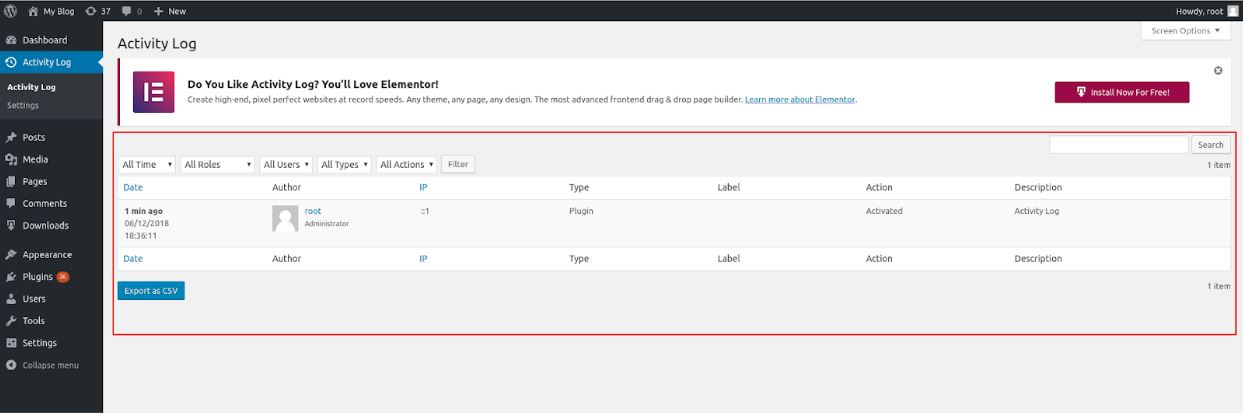
\includegraphics[scale=0.25]{img/admin_view.JPG}
	\caption{Admin-view of a WordPress website, the section enclosed in red is dictated by the plugin code.}
	\label{fig:admin_view}
\end{figure}

\begin{figure}[h]
	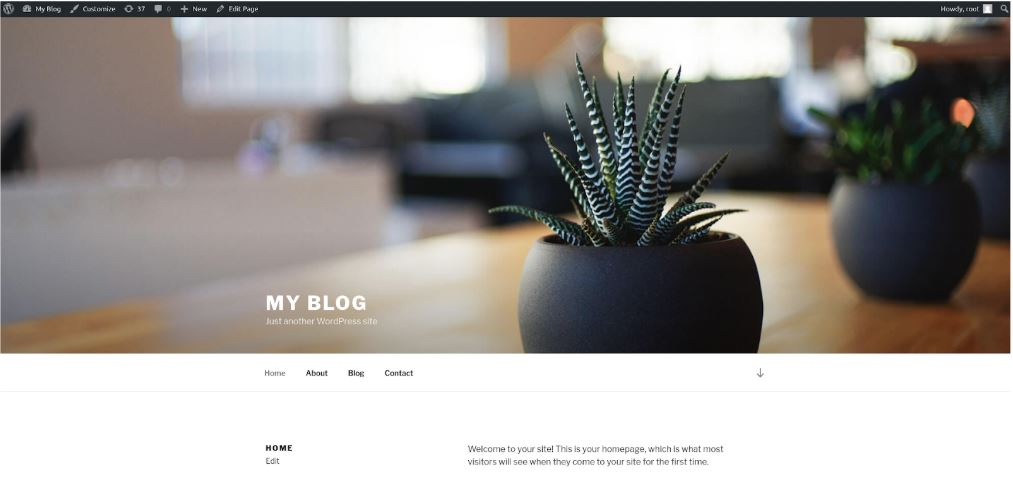
\includegraphics[scale=0.3]{img/user_view.JPG}
	\caption{User view of a WordPress website, much of the layout can be modified by an admin.}
	\label{fig:user_view}
\end{figure}

\subsection{Study Methodology}
In order to achieve a comprehensive study, we have analyzed the 100 most recent CVEs related to XSS attacks, and in particular, to WordPress. We have chosen WordPress because it is widely used (WordPress powers 30\% of the Internet according to a recent survey \cite{w3stats}), and because it is relatively efficient and easy to reproduce many of the attacks related to it: WordPress plugins are very popular among developers and there's many of these that have been found to be vulnerable to XSS; using one framework, we can install many different plugins for the version we want, reproduce attacks, and investigate the conditions under which they happen, without having to install additional software. We have chosen to use a CVE database, as opposed to other databases that include vulnerabilities or exploits, mainly because of reliability. We have been able to find hundreds of verified attacks on WordPress and its plugins using a CVE database, which also usually contain information on how to reproduce them. This provides the perfect platform to analyze XSS attacks and decide whether they can be countered by our approach. 

We tagged the analyzed CVEs with four main pieces of information in a yes/no format:
\begin{itemize}
	\item Whether they can be exploited without privileged user authentication: most WordPress sites will allow users to register, and admins of these sites can give increasingly more important privileges to them. Many exploits rely on the fact that the attacker has enough privileges to, for example, submit a post or change some website configurations. As such, we have decided to mark whether an attack requires the user to have high privileges or could just be an unauthenticated or have the most basic level of registration. 
	\item Whether the attack manifests itself on an admin-only view: As discussed earlier, our approach relies on very specific knowledge of what the HTML document should look like without any code injections. Many WordPress plugins have an admin-only view for configuration setup where XSS manifests itself. These are of particular interest because these views do not change across different installations of the plugin, that is, different websites using the same plugin will display the same HTML in these views, and so our approach will be easier to apply.
	\item Whether the attack manifests itself on a user-only view: Similarly to 2, many XSS attacks on WordPress only manifest themselves on the user side of the website, thus, these are likely to vary across different webpages, even if the attack is caused by a WordPress plugin. However, it's worth mentioning that even if this is the case, all might not be lost, as the attack might happen in a very specific HTML context related to the WordPress plugin.
	\item Whether the attack manifests itself through some HTML element: Sometimes an XSS attack is not tightly linked to the HTML document, it might just be triggered through a POST request by clicking on a link. Attacks that are not related to HTML are not usually covered by our approach. We might be able to use some heuristics for simpler attacks, like URL filtering, but in general we do not expect to be able to guard against these.
\end{itemize}

\subsection{Study Results}

We classified 79 CVEs from our original 100. We dropped 21 of them due to insufficient information in the CVE descriptions to get any meaningful information, or because the plugin code was no longer available. In some cases, the plugin had been removed from the WordPress repository due to "security issues", which exacerbates the importance of being able to defend against these attacks.  

The plugins we studied averaged 489,927 installations (min: 10, max: 5 million). Table~\ref{table:1} reports our main results according to our discussed methodology. It is clear from the results that our approach applies to a majority of the studied CVEs. Of particular importance are the first three reported figures.

 A 72\% in "No Authentication" implies that most attacks can be realized by an outsider, and is an alarming reflection of the current state of browser and application defenses against XSS. 
 
 The "User View Only" represents the hardest scenario for us to defend against XSS, as many of the elements in this view won't persist across different websites. A 14\% here means that only a small minority of plugins won't be able to benefit from our strategy. It is worth noting that we have tagged webpages according to this criterion by barely being displayed in the user view, however, there might still be enough identifying information for the injection  to be defended against, and this number might therefore not be fully representative of the limitations of our approach.
 
  While we report a 66\% in "Admin View Only", in our studies we noted that some of the CVE descriptions were somewhat limited and in some cases weren't accurate in describing where the injection points were rendered. As an example, one CVE explained how an unsanitized parameter could trigger XSS in a specific URL of the admin panel, but we found that there were other parts of the admin panel where the same XSS was being triggered. While we believe that this doesn't pose a big issue since it just counts as a failure of the signature description in the firewall, we note that the actual number of websites that can benefit from our approach might be slightly different. 
 
 Finally, even for plugins where we didn't consider it to be able to be defended against in the admin view, we still report the ones where we believe there is some HTML Context that identifies the injection point and can be used to defend against XSS; however, these might be more prone to false positives and therefore only consider them as a "last resort".

Many of the studied CVEs included attacks for which there are known and widely deployed defenses. For example, many were cases of Reflected XSS, where the URL reveals the existence of an attack e.g:


$http://[path to WordPress]/wp-admin/admin.php?page=wps\_pages\_page\&page-uri=<script>alert("XSS")</script>$

While Firefox didn't block this request, Chrome's built-in XSS auditor did block it. We believe such solutions are important and are complementary to our work, and so we still tagged such attacks as identifiable by our approach, as well as having the ability to detecting them in an extension.

\begin{table}
\begin{center}
	\begin{tabular}{|p{2cm}|p{1.5cm}|p{1.5cm}|p{1.5cm}|} 
		\hline
		No Authentication & Admin View Only & User View Only & HTML Context \\ [1ex] 
		\hline
		57 (72\%) & 52 (66\%) & 11 (14\%) & 71 (89\%) \\  [1ex] 
		\hline
	\end{tabular}
\caption{Study results}
\label{table:1}
\end{center}
\end{table}
